\documentclass{standalone}

\RequirePackage[T1]{fontenc} \RequirePackage[tt=false, type1=true]{libertine}
\RequirePackage[varqu]{zi4} \RequirePackage[libertine]{newtxmath}

\pdfoutput=1

\usepackage{amsfonts}
\usepackage{tikz}
\usetikzlibrary{arrows.meta}

\begin{document}


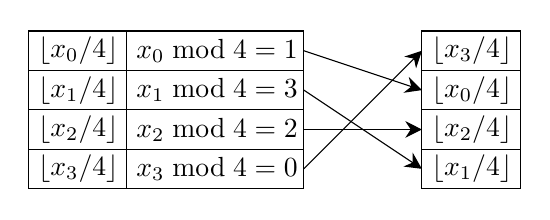
\begin{tikzpicture}

\draw(0,0)   node[right] {$\lfloor x_3/4 \rfloor$};
\draw(0,0.5) node[right] {$\lfloor x_2/4 \rfloor$};
\draw(0,1)   node[right] {$\lfloor x_1/4 \rfloor$};
\draw(0,1.5) node[right] {$\lfloor x_0/4 \rfloor$};

\draw(1.25,0)   node[right] {$x_3 \bmod 4 = 0$};
\draw(1.25,0.5) node[right] {$x_2 \bmod 4 = 2$};
\draw(1.25,1)   node[right] {$x_1 \bmod 4 = 3$};
\draw(1.25,1.5) node[right] {$x_0 \bmod 4 = 1$};

\draw (0,1.75) rectangle (3.5,-0.25);
\draw (0,1.25) rectangle (3.5,0.25);
\draw (0,0.75) -- (3.5,0.75);
\draw (1.25,-0.25) -- (1.25,1.75);

\draw(5,0)   node[right] {$\lfloor x_1/4 \rfloor$};
\draw(5,0.5) node[right] {$\lfloor x_2/4 \rfloor$};
\draw(5,1)   node[right] {$\lfloor x_0/4 \rfloor$};
\draw(5,1.5) node[right] {$\lfloor x_3/4 \rfloor$};

\draw (5,1.75) rectangle (6.25,-0.25);
\draw (5,1.25) rectangle (6.25,0.25);
\draw (5,0.75) -- (6.25,0.75);

\draw [-{Stealth[length=6, width=6]}] (3.5,1.5) -- (5,1);
\draw [-{Stealth[length=6, width=6]}] (3.5,1)   -- (5,0);
\draw [-{Stealth[length=6, width=6]}] (3.5,0.5) -- (5,0.5);
\draw [-{Stealth[length=6, width=6]}] (3.5,0)   -- (5,1.5);

\end{tikzpicture}

\end{document}
